% Abstract Jan 13; Submission Jan 16; Rebuttal Feb 19-21; Notification Mar 14; Camera-ready: Apr 14
% Submisison guidelines: https://hpcrl.github.io/ICS2025-webpage/for-authors/information.html
% Submission site: https://ics25.hotcrp.com/
% 11 pages plus unlimited references; no appendices; double blind
% TODO: metadata of the submitted PDF files should not reveal authors
% TODO: make sure all authors have submitted their conflicts of interest in HotCRP *early*
\documentclass[sigconf, screen, review]{acmart}
\setcopyright{none} 
\copyrightyear{2025}
\acmYear{2025}
\acmDOI{XXXXXXX.XXXXXXX}
\acmConference[SC 2025]{SC 2025}{Nov 16--21, 2025}{St. Louis, MO, USA}
\acmISBN{000-0-0000-0000-0/00/00}
\settopmatter{printfolios=true}
\settopmatter{printacmref=false}

%includes
\usepackage{amsmath}
\usepackage[lined, boxed, ruled, noend]{algorithm2e}
\usepackage{hyperref}
\usepackage{cleveref}
\usepackage{multirow}
\usepackage{xspace}
% \usepackage{algpseudocode}

\usepackage{xcolor}
\usepackage{subcaption}
\usepackage{pgfplots}
\usepackage{pgfplotstable}
\pgfplotsset{compat=1.3}
\usepackage{float}
\usepackage{enumitem}
\setitemize{leftmargin=*,noitemsep,topsep=0pt,parsep=0pt,partopsep=0pt}

\newcommand{\para}[1]{\smallskip\noindent\textbf{#1.}}
\renewcommand{\paragraph}[1]{\para{#1}}

\newcommand{\ps}[1]{{\color{red} Saday: #1}}
\newcommand{\pp}[1]{{\color{red} Prashant: #1}}
\newcommand{\ourtool}{FaSTCC\xspace}


\begin{document}
\title{FaSTCC: Fast Sparse Tensor Contractions on CPUs}
%\begin{abstract}

Sparse tensor contractions are a core computational primitive in scientific computing and machine learning. 
Effective optimization of such contractions through loop permutation/tiling remains an open challenge.
Our work perform the first comprehensive comparative analysis of data access costs and memory requirements for loop permutations for sparse tensor contractions. Based on these insights, we develop FaSTCC, a novel hashing-based parallel implementation of sparse tensor contractions. FaSTCC introduces a new 2D tiled contraction-index-outer scheme and a corresponding tile-aware design. Using probabilistic modeling, our approach automatically chooses between dense and sparse output tile accumulators and selects suitable tile size. We evaluate FaSTCC across two CPU platforms and a range of real-world workloads, demonstrating significant speedups on benchmarks from FROSTT and from quantum chemistry.

%remains a challenge. Existing frameworks like TACO and Sparta are limited by their reliance on fixed loop orders and lack of loop tiling. In this work, we present \ourtool, a high-performance sparse tensor contraction library that explores all three loop orderings and introduces a novel 2D tiled contraction-index-outer scheme. By combining this loop order with a tile-aware design and a model-driven selection of dense or sparse accumulators, \ourtool achieves significant performance gains over the state of the art. We evaluate FaSTCC across two CPU platforms and a range of real-world tensor workloads, demonstrating speedups of up to $11\times$ on benchmarks from FROSTT and quantum chemistry.

% Sparse tensor contractions (SpTCs), a generalization of matrix multiplication, are critical in applications such as machine learning, quantum chemistry and physics. ...
\end{abstract}
\maketitle

\newcommand{\scaddition}[1]{\textcolor{blue}{#1}}

\newcommand{\hunterinline}[1]{\todo[inline, size=\tiny,color=pink]{Hunter: #1}}

\pgfplotsset{
  barChart/.style={
        small,
        ybar,
        clip=true,
        width = \columnwidth,
        height =.5\columnwidth,
        bar width=0.25cm,
        ymajorgrids, tick align=inside,
        major grid style={draw=white},
        % enlarge y limits={value=.1,upper},
        enlarge x limits={0.15},
        % x=2.5cm,
        ymin=0.1,
        axis x line*=bottom,
        axis y line*=left,
        y axis line style={opacity=0},
        % tickwidth=0pt,
        % enlarge x limits=true,
        ylabel={Speedup},
        %symbolic x coords={
        %   init,insert,insertRange,delete,
        %   deleteRange},
       xtick=data,
       legend pos = outer north east,
       point meta=rawy,
       nodes near coords,
       every node near coord/.append style={rotate = 90, anchor = west, font=\scriptsize	,/pgf/number format/fixed relative,/pgf/number format/precision=2},
        x tick label style={rotate=-35,anchor=west, yshift=-2pt}
  }
}

\pgfplotsset{
  barChartSmall/.style={
        small,
        ybar,
        clip=true,
        width = \columnwidth,
        height =.4\columnwidth,
        bar width=0.25cm,
        ymajorgrids, tick align=inside,
        major grid style={draw=white},
        % enlarge y limits={value=.1,upper},
        enlarge x limits={0.15},
        % x=2.5cm,
        ymin=0.1,
        axis x line*=bottom,
        axis y line*=left,
        y axis line style={opacity=0},
        % tickwidth=0pt,
        % enlarge x limits=true,
        ylabel={Speedup},
        %symbolic x coords={
        %   init,insert,insertRange,delete,
        %   deleteRange},
       xtick=data,
       legend pos = outer north east,
       point meta=rawy,
       nodes near coords,
       every node near coord/.append style={rotate = 90, anchor = west, font=\scriptsize	,/pgf/number format/fixed relative,/pgf/number format/precision=2},
        x tick label style={rotate=-35,anchor=west, yshift=-2pt}
  }
}

\pgfplotsset{
  barChartScaling/.style={
        small,
        ybar,
        clip=true,
        width = \columnwidth,
        height =.4\columnwidth,
        bar width=0.25cm,
        ymajorgrids, tick align=inside,
        major grid style={draw=white},
        % enlarge y limits={value=.1,upper},
        enlarge x limits={0.15},
        % x=2.5cm,
        ymin=0.1,
        axis x line*=bottom,
        axis y line*=left,
        y axis line style={opacity=0},
        % tickwidth=0pt,
        % enlarge x limits=true,
        ylabel={Speedup},
        %symbolic x coords={
        %   init,insert,insertRange,delete,
        %   deleteRange},
       xtick=data,
       legend pos = outer north east,
       point meta=rawy,
       nodes near coords,
       every node near coord/.append style={rotate = 90, anchor = west, font=\scriptsize	,/pgf/number format/fixed relative,/pgf/number format/precision=2},
        x tick label style={anchor=north, yshift=-2pt}
  }
}

\pgfplotsset{
  tacoBarChart/.style={
        small,
        ybar,
        clip=true,
        width = \columnwidth,
        height =.4\columnwidth,
        bar width=0.25cm,
        ymajorgrids, tick align=inside,
        major grid style={draw=white},
        % enlarge y limits={value=.1,upper},
        enlarge x limits={0.15},
        % x=2.5cm,
        ymin=0.1,
        axis x line*=bottom,
        axis y line*=left,
        y axis line style={opacity=0},
        % tickwidth=0pt,
        % enlarge x limits=true,
        ylabel={Speedup},
        %symbolic x coords={
        %   init,insert,insertRange,delete,
        %   deleteRange},
       xtick=data,
       legend pos = outer north east,
       point meta=rawy,
       nodes near coords,
       every node near coord/.append style={rotate = 90, anchor = west, font=\scriptsize	,/pgf/number format/fixed relative,/pgf/number format/precision=2},
        x tick label style={rotate=-35,anchor=west, yshift=-2pt}
  }
}

\pgfplotsset{
ScatterPlot/.style={
    small,
    width = \columnwidth,
    height = \columnwidth/2,
    table/col sep=comma,
    unbounded coords=jump,
    xtick={32,64,128,256,362,512,724,1024,2048},
    %enable this for rotated sizes
    xticklabels={32,64,128,256,362,512,724,1024,2048},
    log basis x=2,
    x tick label style={font=\normalsize, rotate=35, anchor=east, yshift=-2pt},
    %enable this for number 4-12 
    %xticklabel={\pgfmathfloatparsenumber{\tick}\pgfmathprintnumber{\pgfmathresult}},
    %xticklabels from table={\datatable}{Bytes},
    %each nth point=2,
    x tick label style={font=\normalsize},
    legend pos = outer north east,
    xlabel={Tile Size},
    ylabel={Execution time (S)}
    }
}

\pgfplotsset{
moleculeScatterPlot/.style={
    small,
    width = \columnwidth,
    height = \columnwidth/2,
    table/col sep=comma,
    unbounded coords=jump,
    xtick={32,64,128,256,512,1024,2048},
    %enable this for rotated sizes
    xticklabels={32,64,128,256,512,1024,2048},
    log basis x=2,
    x tick label style={font=\normalsize, rotate=35, anchor=east, yshift=-2pt},
    %enable this for number 4-12 
    %xticklabel={\pgfmathfloatparsenumber{\tick}\pgfmathprintnumber{\pgfmathresult}},
    %xticklabels from table={\datatable}{Bytes},
    %each nth point=2,
    x tick label style={font=\normalsize},
    legend pos = outer north east,
    xlabel={Tile Size},
    ylabel={Execution time (S)}
    }
}

\definecolor{lightBlue}{HTML}{9ABDDC}



%NIPS-013	Chicago-0	Chicago-01	Chicago-123	Vast-5d-01	Vast-5d-014	Uber-02	Uber-123

  

\pgfplotsset{
  NIPS013/.style     = {color = magenta,  mark = square*},
  Chicago0/.style     = {color = orange,       mark = triangle*},
  Chicago01/.style     = {color = orange,       mark = diamond*},
  Chicago123/.style     = {color = orange,       mark = pentagon*},
  Vast01/.style     = {color = lightBlue,       mark = square*},
  Vast014/.style     = {color = magenta,       mark = pentagon*},
  Uber02/.style     = {color = red,       mark = triangle*},
  Uber123/.style     = {color = red,       mark = pentagon*},
  RedBarStyle/.style = {fill = red},
  OrangeBarStyle/.style = {fill = orange},
  BlueBarStyle/.style = {fill=lightBlue},
}


%\input{introduction}
%\section{Background}
\label{sec:background}
%\ps{Section is not flowing well; moving related work to the end of the paper.}
\subsection{Sparse Tensor Contractions}
A tensor $T$ of order $n$ is defined by a set of $n$ modes, with mode $M_k = \{ 1, \ldots, N_k\}$ for $1 \le k \le n$. These modes define the index space of the tensor. $T_{i_1,\ldots,i_n}$ denotes the tensor element for a particular point in that index space, with $i_k\in M_k$. 
%\emph{index space} $D_1 \times \ldots \times D_n$; here $n$ is the tensor mode. Each set $D_i$ in this Cartesian product defines a set of index values $\{1,\ldots,N_i\}$. For a tensor $T$ of mode $n$, $T_{i_1,\ldots,i_n}$ denotes the tensor element for index point $\langle i_1, \ldots, i_n\rangle$. 
In a \emph{sparse tensor} most $T_{i_1,\ldots,i_n}$ have zero numeric values; thus, standard dense representations of size $\prod_k N_k$ are wasteful. Instead, compact representations such as COO (COOrdinate format \cite{tewarson1973sparse,frostt_page}) or CSF (Compressed Sparse Fiber \cite{smith-csf}) are used. 

Consider two tensors $L$ and $R$. A \emph{tensor contraction} of $L$ and $R$ is a tensor $O$ defined by
$$O_{l_1,\ldots,l_p,r_1,\ldots,r_q} = \sum_{c_1,\ldots,c_m} L_{l_1,\ldots,l_p,c_1,\ldots,c_m} \ast R_{c_1,\ldots,c_m, r_1,\ldots,r_q}$$
Here \emph{contraction indices} $c_1,\ldots,c_m$ denote modes that are common to both tensors. These contraction indices are specified as part of the contraction definition. The remaining indices $l_1,\ldots,l_p$ and $r_1,\ldots,r_q$ are referred to as \emph{external indices}.

Clearly, this is a higher-dimensional analog of matrix-matrix multiplication. In fact, the approach we define in this paper assumes that a pre-processing step has been applied to linearize the tuple $l_1,\ldots,l_p$ to a single index $l\in \mathbb{L}$. Similarly, $r_1,\ldots,r_q$ is linearized to an index $r\in \mathbb{R}$ and $c_1,\ldots,c_m$ is linearized to an index $c\in \mathbb{C}$. In our implementation such linearlization is applied as a pre-processing step, and the inverse delinearlization is applied as a post-processing step (both are accounted for in the measured execution time). Thus, the computation we aim to optimize is 
$$O_{lr} = \sum_c L_{lc} \ast R_{cr}, \ l \in \mathbb{L}, r \in \mathbb{R}, c\in \mathbb{C}$$
%with ranges $l\in \mathbb{L}$, $r \in \mathbb{R}$, and $c\in \mathbb{C}$. 

Application domains that use tensor contractions (e.g., physics and chemistry) often employ the Einstein notation.
For the contraction shown above, this notation is $O_{lr} = L_{lc}R_{cr}$. Since the tensor modes corresponding to external and contraction indices are explicitly specified in a tensor contraction, in Einstein notation the relative order of indices 
%that index a tensor 
does not have any significance to the semantics of the contraction. All of the following are mathematically equivalent: $O_{lr} = L_{lc}R_{cr}; O_{lr} = L_{lc}R_{rc}$; $O_{rl} = L_{lc}R_{rc}$; $O_{lr} = R_{rc}L_{lc}$. % $O_{rl} = R_{rc}L_{lc}$. 

%-- Define tensor contractions in Einstein notation and relate to matrix-matrix multiplication, explaining linearized indices for external and contraction dimensions.
%-- Define notation $\mathbb{L}, \mathbb{R}, \mathbb{C}$

\subsection{Sparse Tensor Representations}

A variety of representations for sparse tensors have been considered in prior efforts. We outline the most relevant three representations. 

The COO (Coordinate) format~\cite{tewarson1973sparse} stores a sparse tensor as a list of tuples, each of which 
describes a nonzero tensor element. For a tensor with $n$ modes, each tuple contains $n+1$ values, with the first $n$ values representing index coordinates
%corresponding to each of the N dimensions 
and the final one representing the numeric value of the tensor element. While the COO format is not as compact as other formats, it does support constant-cost insertions of new elements, since a new tuple can simply be appended to the end of the list. Due to its ease of construction COO is commonly used to read in input tensors and write out result tensors, with the tensor being converted from COO to a more optimized format for the targeted computations. Both Sparta \cite{liu2021sparta} and \ourtool\ consume COO input and produce COO output.

The CSF (Compressed Sparse Fiber) format \cite{smith-csf} is based on a chosen outer-to-inner order of the tensor modes. CSF structures a sparse tensor as a tree. The internal nodes of this tree at a depth $k$ represent the indices present in the $k$-th mode, and each leaf in the tree represents one nonzero element in the tensor.
%At each level of this hierarchical layout, a subset of the indices for the corresponding mode is represented, based on the sparsity structure of the tensor. Efficient iteration over hyper-rectangular tensor slices requires an iteration order consistent with the hierarchical CSF layout.

%Hash tables:

Some approaches (e.g., Sparta \cite{liu2021sparta}) employ hash tables to represent sparse tensors. A hash table
%are a fundamental data structure that 
maps a universe of keys to a universe of values. Internally, hash tables store keys by mapping them to an internal slot via a \emph{hash function}, a function that deterministically maps input data to an output universe of a fixed size. Hash tables come in two categories, \textit{open addressing} and \textit{closed addressing} (or \emph{chaining}). Open addressing tables use a hash function to map input keys to positions in a fixed size array: if the position chosen for a key is occupied, the key finds a new position via a probing scheme that determines which positions to probe in the array. Closed addressing schemes hash keys to a bucket data structure which can store any number of keys using chaining (or linked list). The chaining table used in Sparta is one such table, as keys are mapped to an internal linked list during insertion.
Open addressing hash tables can achieve higher space efficiency and offer better data locality compared to chaining hash tables.

%TODO - discuss robin hood hashing - hash order and whatnot.
%\section{Analysis of Loop Orders for Sparse Tensor Contraction}
\label{sec:looporder}

% {\color{red} {\bf Expand the analysis to be more comprehensive and include tiling. We should make sure to address the following from the ICS'25 reviews:}
% \begin{itemize}
%     \item Incomplete Analysis: The analysis in this paper only considers the queries and data volume for the input tensors, without taking into account the accumulation from the workspace to the output tensor. While the queries and data volume of the CO method for the input tensors might be smaller than those of CI and CM, this may not hold true when considering the queries and data volume between the workspace and the output tensor.
% \end{itemize}
% }
%{\color{red}Hunter: TACO doesn't appear to be mentioned in section~\ref{sec:background}.}

%{\color{blue}Saday: Thanks for catching that, Hunter. We moved the TACO description to the Related Work at the end. Will delet the mention here.}
%In Section~\ref{sec:background}, two state-of-the-art approaches for sparse tensor contraction were summarized: the TACO compiler~\cite{kjolstad-oopsla17}  and the Sparta library~\cite{liu2021sparta}. 

In this section, we perform a comparative analysis of the data access costs for sparse tensor contraction for different {\em loop orders}. We first perform the analysis without considering tiling, and then in Section~\ref{sec:tile-analysis} extend the analysis for the tiled case.

 
%(without considering specific sparse tensor representations)
A sparse tensor contraction is shown in an abstract form in Algorithm~\ref{algo:abstract-sptc}, using the notation from Section~\ref{sec:background}.

\begin{algorithm}[h]
\DontPrintSemicolon
\LinesNumbered
\For{$l \in \mathbb{L}$}{
  \For{$c \in \mathbb{C}$ with nonzero $L_{lc}$}{
    \For{$r \in \mathbb{R}$ with nonzero $R_{rc}$}{
      $O_{lr} \gets O_{lr} + L_{lc} \ast R_{rc}$}}}
\caption{Abstract Sparse Tensor Contraction\label{algo:abstract-sptc}}
\end{algorithm}

%As noted earlier, the ordering of indices used to access a tensor does not affect the semantics of a tensor contraction. 
%The abstract formulation of sparse tensor contraction can be expressed using any of the six possible permutations of the loops over $c$, $l$, and $r$.
%The choice of tensor representations significantly impacts performance, making loop order a critical design consideration.

%Since the tensor modes corresponding to external and contraction indices are explicitly identified in a tensor contraction, 
% As discussed earlier, the relative order of indices that index a tensor does not have any significance to the semantics of a tensor contraction. 
%For example, all of the following are mathematically equivalent: $O_{lr} = L_{lc}R_{rc}$; $O_{rl} = L_{lc}R_{rc}$; $O_{lr} = R_{rc}L_{lc}$; $O_{rl} = R_{rc}L_{lc}$. 
% Further, the above abstract specification of sparse tensor contraction could be specified via any of the 6 possible permutations of the loops over $c$, $l$, and $r$. However, for any concrete implementation of sparse tensor contraction, the specific representations used for the tensors have strong implications on performance.  

In the compressed sparse fiber (CSF) representation, tensor indices are typically ordered from left to right according to the outer-to-inner hierarchy, defining the tensor’s layout. This means that efficient element access is possible 
only for loop orders that align with the tensor’s layout: accessing elements in non-layout-compatible order requires costly searches. In contrast, using a hash table to store sparse tensor elements allows flexible and efficient access across different loop orders, depending on how the table is indexed. 

Since the roles of the two input tensors (``left'' or ``right'') are interchangeable in a contraction, only three unique loop orders need to be considered — determined by the position of the contraction index in the loop nest. Below, we examine these three loop orders and analyze their impact on data access costs in sparse tensor contractions.
For each case, we first create appropriately indexed hash tables for the two input tensors.
%and discuss the options for handling the accumulations for the sparse output tensor.


% With a compressed sparse fiber (CSF) representation, the usual convention is that the left-to-right order of indexing a tensor corresponds to the outer-to-inner hierarchical representation, or {\em layout} of the tensor. With a CSF representation, only nested loop orders that match the layout-order of a tensor can be used for efficient access to tensor elements, and random access with respect to any index will require expensive search. However, by using a hash table to hold the elements of a sparse tensor, by suitably indexing the hash table, efficient tensor access for different loop orders is feasible. Of the 6 possible loop orders for sparse tensor contraction, since it is completely equivalent to label either of the two input tensors as the ``left'' or ``right'' tensor, there are only three distinct loop orders to consider, corresponding to the position of the contraction index in the nested loop order. Below, we discuss each of the three loop orders, and analyze them in terms of the implications for data access costs in performing sparse tensor contraction. 



%%%%%%%%%%%%%%%%%%%%%%%%%%%%%%%%%%%%%%%%%%%%%%
\subsection{Contraction-Inner (CI) Scheme } 
The input tensors are first placed in hash tables as follows:
$$\mathit{HL}: \mathbb{L} \rightarrow \mathcal{P}(\mathbb{C} \times \mathbb{V})$$
$$\mathit{HR}: \mathbb{R} \rightarrow \mathcal{P}(\mathbb{C} \times \mathbb{V})$$

$\mathbb{L}$ is the set of values for the left index $l$ (assuming linearization if there are multiple left indices $l_1, l_2, \ldots$). Similarly, $\mathbb{R}$ is the set of values for the right index $r$ and $\mathbb{C}$ is the set of values for the contraction index $c$. The numeric values are from set $\mathbb{V}$. We use $\mathcal{P}(X)$ denotes the powerset of $X$. 

For each possible combination of $l$ and $r$, this scheme requires the determination of the intersection of $\mathit{HL}(l)$ and $\mathit{HR}(r)$ in order to find pairs $\langle c,\mathit{lv} \rangle$ and $\langle c,\mathit{rv} \rangle$ with matching values of $c$. 

\begin{algorithm}[h]
\DontPrintSemicolon
\LinesNumbered
\For{$l \in \mathbb{L}$}{
   \For{$r \in \mathbb{R}$}{
   $\mathit{sum} \gets 0$ \;
   $\mathit{update} \gets \mathit{false}$ \;
   \For{$\langle c,\mathit{lv} \rangle \in \mathit{HL}(l) \wedge \langle c,\mathit{rv} \rangle \in \mathit{HR}(r) $}{
      $\mathit{sum} \gets \mathit{sum} + \mathit{lv} \ast \mathit{rv}$ \;
      $\mathit{update} \gets \mathit{true}$ }
   \If{$\mathit{update}$}{$\mathit{Out}.\mathit{append}(l, r, \mathit{sum})$} } }
\caption{Contraction-Inner (CI)\label{algo:ci}}
\end{algorithm}

%Details of efficient set intersection are not discussed below.
%A simple solution is to represent each set as a sequence of pairs $\langle c,v \rangle$ sorted by $c$, which requires $\mathcal{O}(n\log{}n)$ cost when $\mathit{HL}$ and $\mathit{HR}$ are constructed, but has linear cost for determining the intersection. 
With this scheme (Algorithm~\ref{algo:ci}), the output tensor is constructed element-by-element by using a scalar variable $sum$ to accumulate all contributions from matching pairs of nonzero elements from the two inputs.
The TACO compiler \cite{kjolstad-oopsla17} can automatically synthesize efficient tensor contraction code for the CI scheme, using CSF representations of the input tensors, where the contraction index is innermost in both input tensors. This scheme is therefore also called an ``inner-inner" scheme. 
%CSF structures allow a similar kind of index space mapping as the hashtable $\mathit{HL}: \mathbb{L} \rightarrow \mathcal{P}(\mathbb{C} \times \mathbb{V})$.
A CSF mode order with outer mode $\mathbb{L}$ and inner mode $\mathbb{C}$ allows iteration over $l$ followed by $c$.
In contrast to a hash table, CSF needs sorted indices in every dimension, and cannot resize dynamically. The cost of creating CSF is therefore $O(\mathit{nnz}\ast \log(\mathit{nnz}))$ where $\mathit{nnz}$ is the number of nonzero elements.
Furthermore, to obtain a nonzero value, this approach needs lookups in $2\times n$ arrays where $n$ is the order of the tensor. 
%Hash tables usually offer lookups in a few (up to 2 in most practical implementations) cache line loads.

%%%%%%%%%%%%%%%%%%%%%%%%%%%%%%%%%%%%%%%%%%%%%%

\subsection{Contraction-Middle (CM) Scheme} 
\label{subsec:contraction-middle}
The input tensors are first placed in hash tables as follows:
$$\mathit{HL}: \mathbb{L} \rightarrow \mathcal{P}(\mathbb{C} \times \mathbb{V})$$
$$\mathit{HR}: \mathbb{C} \rightarrow \mathcal{P}(\mathbb{R} \times \mathbb{V})$$

\begin{algorithm}[h]
\DontPrintSemicolon
\LinesNumbered
\For{$l \in \mathbb{L}$}{
  $\mathit{WS} \gets \emptyset$ \;
  \For{$\langle c,\mathit{lv} \rangle \in \mathit{HL}(l)$}{
    \For{$\langle r,\mathit{rv} \rangle \in \mathit{HR}(c)$}{
      $\mathit{WS}.\mathit{upsert}(r,\mathit{lv} \ast \mathit{rv})$ \; }}
  \For{$r \in \mathit{WS}.\mathit{keys}$}{
    $\mathit{Out}.\mathit{append}(l, r, \mathit{WS}(r))$ } }
\caption{Contraction-Middle (CM)\label{algo:cm}}
\end{algorithm}
In Algorithm~\ref{algo:cm}, the contraction index iterates in the middle loop. For each index $l \in  \mathbb{L}$, all nonzero elements $L_{lc}$ with external index $l$ are extracted from the hash table $\mathit{HL}$.
For each value $c$, 
% from these nonzeros, 
nonzero elements $R_{cr}$ are extracted from hash table $\mathit{HR}$ by using $c$ as the key. The product $L_{lc}R_{cr}$ is a contribution to $O_{lr}$. Accumulations to $O_{lr}$ must be performed for each extracted $R_{cr}$. This must be done for all $c$ corresponding to nonzero elements $L_{lc}$. 
%Since the order of accumulations to the various $O_{lr}$ for different values of $c$ can be arbitrary (depends on the nonzero patterns in $R_{cr}$), 
A workspace $\mathit{WS}$ is used for performing the accumulations to the appropriate output elements $O_{l*}$:
$$\mathit{WS}: \mathbb{R} \rightarrow \mathbb{V} $$ Either a dense array (along with some auxiliary data structures to keep track of which elements of the workspace are updated and become nonzero) or a sparse accumulator (using a hash table) may be used for $\mathit{WS}$.
 Update operation $\mathit{WS}.\mathit{upsert}(r,v)$ modifies the workspace as follows: if $r \notin \mathit{WS}.\mathit{keys}$, $\mathit{WS}(r)$ is set to $v$; otherwise, $v$ is added to $\mathit{WS}(r)$. 

%%%%%%%%%%%%%%%%%%%%%%%%%%%%%%%%%%%%%%%%%%%%%%
\subsection{Contraction-Outer (CO) Scheme} 
The input tensors are represented as follows:
$$\mathit{HL}: \mathbb{C} \rightarrow \mathcal{P}(\mathbb{L} \times \mathbb{V})$$
$$\mathit{HR}: \mathbb{C} \rightarrow \mathcal{P}(\mathbb{R} \times \mathbb{V})$$
In addition, a 2D workspace is used: 
$$\mathit{WS}: (\mathbb{L} \times \mathbb{R}) \rightarrow \mathbb{V} $$
The workspace $\mathit{WS}$ has keys that are pairs $\langle l, r \rangle \in \mathbb{L} \times \mathbb{R}$.

\begin{algorithm}[h]
\DontPrintSemicolon
\LinesNumbered
$\mathit{WS} \gets \emptyset$ \;
\For{$c \in \mathbb{C}$}{
  \For{$\langle l,\mathit{lv} \rangle \in \mathit{HL}(c)$}{
    \For{$\langle r,\mathit{rv} \rangle \in \mathit{HR}(c)$}{
      $\mathit{WS}.\mathit{upsert}(l,r,\mathit{lv} \ast \mathit{rv})$ \; } }}
\For{$\langle l, r \rangle \in \mathit{WS}.\mathit{keys}$}{
    $\mathit{Out}.\mathit{append}(l, r, \mathit{WS}(l,r))$ } 

\caption{Contraction-Outer (CO)\label{algo:co}}
\end{algorithm}

The CO scheme in Agorithm~\ref{algo:co} has the contraction index as the outer loop. Both input tensors have their nonzero elements inserted into hash tables $\mathit{HL}(c)$ and $\mathit{HR}(c)$, indexed by the contraction index. For each value $c$ of the contraction index that has nonzero elements in both $\mathit{HL}(c)$ and $\mathit{HR}(c)$, the product of each $L_{cl}$ and $R_{cr}$ must be formed and accumulated for output element $O_{lr}$. The workspace $\mathit{WS}$ is used to perform the accumulations. Operation $\mathit{WS}.\mathit{upsert}(l,r,v)$ updates the workspace as expected: if $(l,r) \notin \mathit{WS}.\mathit{keys}$, $\mathit{WS}(l,r)$ is set to $v$; otherwise, $v$ is added to $\mathit{WS}(l,r)$.

\subsection{Comparative Analysis of Loop Orders}
We next compare the three schemes with respect to data access costs. For this analysis, we assume a dense workspace for performing accumulations for output tensor elements. For the output tensor, the number of accumulation operations is identical for all three schemes, and the main difference is the size of the workspace (which may in turn affect data access cost, if a small workspace can fit within cache but a large workspace requires DRAM accesses).\\ 
%However, for the input tensors, the three loop orders have very different reuse factors for the input data elements. We contrast two key metrics for the three loop orders.\\
\noindent{\bf Data Access for Input Tensors:} The input tensors are stored and accessed from hash tables. Each query incurs the cost of generating a hash value from the key and an access into the hash table to determine if the key exists. The payload for a successful query is not uniform, being directly proportional to the number of nonzero elements in the accessed slices of the tensor. We therefore separately quantify the number of hash table queries and the total volume (number of nonzero elements) of data retrieved over the full execution of the sparse tensor contraction. 
%\pp{Is $2C$ slice correct?}
%{\color{blue} Saday: I removed the $2C$.}

\noindent{\bf CI:} The CI scheme (Algorithm~\ref{algo:ci}) computes the sparse inner product between every pair of left tensor slice $l \in  \mathbb{L}$ and right tensor slice  $r \in \mathbb{R}$. Thus, $O(L \times R)$ queries to the input hash tables are required, where $L$ and $R$ are the extents of the respective index spaces of $\mathbb{L}$ and $\mathbb{R}$. For each such pair of slices from the left tensor and the right tensor, their nonzero elements must be co-iterated to find elements with matching values of the contraction index $c$. This is done efficiently if the nonzero elements are sorted in increasing value of $c$, but even so the volume of data access is very high: each slice of the right tensor must be accessed for each slice of the left tensor, with a total volume of $O(L \times \mathit{nnz}_R)$, and similarly a volume of $O(R \times \mathit{nnz}_L)$ for the left tensor, where $\mathit{nnz}_L$ and $\mathit{nnz}_R$ denote the number of nonzero elements in the left and right tensor, respectively.\\
\noindent{\bf CM:}  With the CM loop order (Algorithm~\ref{algo:cm}), for each  $l \in  \mathbb{L}$ for the left tensor, the nonzero elements $L_{lc}$ are accessed, along with queries to slices $R_{cr}$ from the right tensor. The number of queries to the left tensor is $L$. Since each nonzero element in $L$ causes a query to the right tensor, the total number of queries to the right tensor is $\mathit{nnz}_L$. The volume of data accessed for the left tensor is $\mathit{nnz}_L$ because each nonzero element in the tensor is accessed once. Each element $R_{cr}$ of the right tensor will be extracted for every nonzero $L_{cl}$. Therefore the total volume of data accessed for the right tensor is $\sum_{c \in \mathbb{C}}{\mathit{nnz}_L(c) \times \mathit{nnz}_R(c)}$, where $\mathit{nnz}_L(c)$ and $\mathit{nnz}_R(c)$ denote the number of nonzero elements is the slices of the tensors for contraction index $c$. This sum can be approximated as $\frac{\mathit{nnz}_L}{C} \times \sum_{c \in \mathbb{C}} \mathit{nnz}_R(c)$ = $\frac{\mathit{nnz}_L \times \mathit{nnz}_R}{C}$.\\
\noindent{\bf CO:} With the CO loop order (Algorithm~\ref{algo:co}), each slice $L_{c*}$ and $R_{c*}$ is only accessed once. The number of hash table queries for the input tensors is $C+C = 2C$; the data volume is $\mathit{nnz}_L + \mathit{nnz}_R$. 

\noindent{\bf Data Access for Output Tensor:} For any of the loop orders, a temporary workspace must be used to accumulate contributions to nonzero output elements. While the size of the required workspace is affected by the loop order, the total number of accesses to the output workspace is independent of the loop order and equals the total number of multiply-accumulate operations.

\noindent{\bf Workspace Size:} The three schemes impose very different demands on the size of the dense workspace. We quantify the space required.\\
\noindent{\bf CI:} The output elements are processed one at a time and therefore only one scalar variable is needed for the workspace.\\
\noindent{\bf CM:} If a dense workspace is used, a 1D array must be used, of size $\mathbb{R}$, i.e., $R$.\\
\noindent{\bf CO:} With a dense workspace, a 2D array will be needed, whose size is the product of the ranges of  $\mathbb{L}$ and $\mathbb{R}$, i.e., $L \times R$.
\begin{table}
    \centering
    \caption{Comparison of data movement and space needed}
    \begin{tabular}{|c|c|c|c|} \hline 
         Scheme&  Queries&  Data Volume&  Size\_Acc \\ \hline 
         CI&  $O(L \times R)$&  $O(L \times \mathit{nnz}_R + R \times \mathit{nnz}_L)$ & $1$   \\ \hline 
         CM&  $L+\mathit{nnz}_L$& $O(\mathit{nnz}_L + \frac{\mathit{nnz}_R \times \mathit{nnz}_L}{C})$ & $R$  \\ \hline 
         CO& $O(2 \times C)$ & $\mathit{nnz}_L + \mathit{nnz}_R$ & $L \times R$  \\ \hline
    \end{tabular}
    \label{tab:compare_loop_orders}
\end{table}

From the description of the schemes for the three loop orders and the analysis above, we can observe the following trade-offs:
\begin{itemize}
    \item The {\em Contraction-Inner (CI)} scheme incurs the highest data access overhead because of lower reuse of data elements of the input tensors. However, the handling of the accumulations for the sparse output tensor is very straightforward and the scheme can be readily implemented for tensors of any dimensionality. 
    %The TACO compiler~\cite{kjolstad-oopsla17} can automatically generate efficient code for the CI scheme for contracting any sparse tensors. 
    %While our description of all schemes used hash tables to hold the input tensors, 
    %TACO directly traverses input tensors in the CSF format (with contraction-index innermost) without needing to use any hash tables.% It requires that both input tensors inherently have the contraction-index innermost.
    \item The {\em Contraction-Middle (CM)} scheme is much more efficient with respect to the number of queries and the volume of data movement for input tensor elements than the CI scheme. However, the handling of accumulations requires a work-space, whose size depends on the extent $R$, for a dense workspace. 
    In the case of very sparse high-dimensional output tensors, a dense workspace may be feasible or inefficient to use
    if the product of the mode extents corresponding to $\mathbb{R}$ is 
    %too large to fit in memory.
    very high. Sparta~\cite{liu2021sparta} implements the CM scheme as described in Section~\ref{sec:sparta}.
    %It assumes both input tensors are in a COO representation and uses sorting on $L$, inserts the nonzero elements into a hash table for $R$, and uses a sparse accumulator for $O$. 
    \item The {\em Contraction-Outer (CO)} scheme is the most efficient in terms of accesses to input tensors. However, the required size for a dense output accumulator is problematic. Furthermore, even if the dense accumulator could fit in DRAM, update operations could be very slow due to the high latency to DRAM. 
    %We are unaware of any current sparse tensor contraction implementation that uses the CO scheme.  
\end{itemize}

%\noindent{\em In this paper, we use tiling to overcome this memory challenge and develop a tiled-CO scheme for sparse tensor contraction. Our results demonstrate that this approach outperforms the existing state-of-the-art CI (generated by TACO \cite{kjolstad-oopsla17,zhang2024compilation}) and CM (Sparta \cite{liu2021sparta}) implementations.}

%{\color{red} \bf ToDo: Add text for  subsection on tiled execution}

\subsection{Tiled CO Scheme}
From the above discussion, the CO loop order has the lowest number of data accesses but faces challenges with the output workspace. This challenge can be overcome by using 2D tiling along the linearized output tensor dimensions, so that the size of the output accumulator can be controlled by the chosen tile sizes.
\begin{algorithm}[h]
\DontPrintSemicolon
\LinesNumbered
Create $\mathit{NL}$ left hash tables: $\mathit{HL_T[lt]}$\\
Create $\mathit{NR}$ right hash tables: $\mathit{HR_T[rt]}$\\
\For {$\mathit{lt} \gets 0$ \KwTo $\mathit{NL} - 1$}{
\For {$\mathit{rt} \gets 0$ \KwTo $\mathit{NR} - 1$}{
Execute\_Tiled\_CO$(\mathit{lt}, \mathit{rt})$
%$\mathit{WS} \gets \emptyset$ \;
%\For{$c \in \mathit{HL}_i.\mathit{keys}$}{
% \If{$c \in \mathit{HR}_j.\mathit{keys}$}{
%   \For{$\langle l,\mathit{lv} \rangle \in \mathit{HL}_i(c)$}{
%     \For{$\langle r,\mathit{rv} \rangle \in \mathit{HR}_j(c)$}{ 
%         $\mathit{WS}.\mathit{upsert}(l,r,\mathit{lv} \ast \mathit{rv})$ \;
%}
%}
%}
%}
}
}

\caption{2D-Tiled CO scheme\label{algo:tiled-co}}
\end{algorithm}

Algorithm~\ref{algo:tiled-co} outlines the 2D-tiled CO scheme. The output tensor's index space $\mathbb{L} \times \mathbb{R}$ is partitioned into ${\mathit{NL} \ast \mathit{NR}}$ tiles, where $\mathit{NL} = \lceil|\mathbb{L}| / \mathit{T_L} \rceil$ and $\mathit{NR} = \lceil|\mathbb{R}| / \mathit{T_R} \rceil$.
Here $\mathit{T_L}$ and $\mathit{T_R}$ are tile sizes, selected as described later in the paper.
The elements of the left input tensor are inserted from the input COO format into $\mathit{NL}$ hash tables, where an element with index $\langle l,c\rangle$ is inserted into hash table $\mathit{HL_T[lt]}$, where $\mathit{lt} = \lfloor \frac{l}{\mathit{TL}}\rfloor$, and similarly for the right input tensor. A total of ${\mathit{NL} \times \mathit{NR}}$ parallel invocations of instances of the 2D-tiled CO algorithm are dynamically scheduled on the available cores. Details are presented in the next section.
%\input{indexing}
%\section{FaSTCC Design and Implementation\label{sec:details}}

\begin{figure}
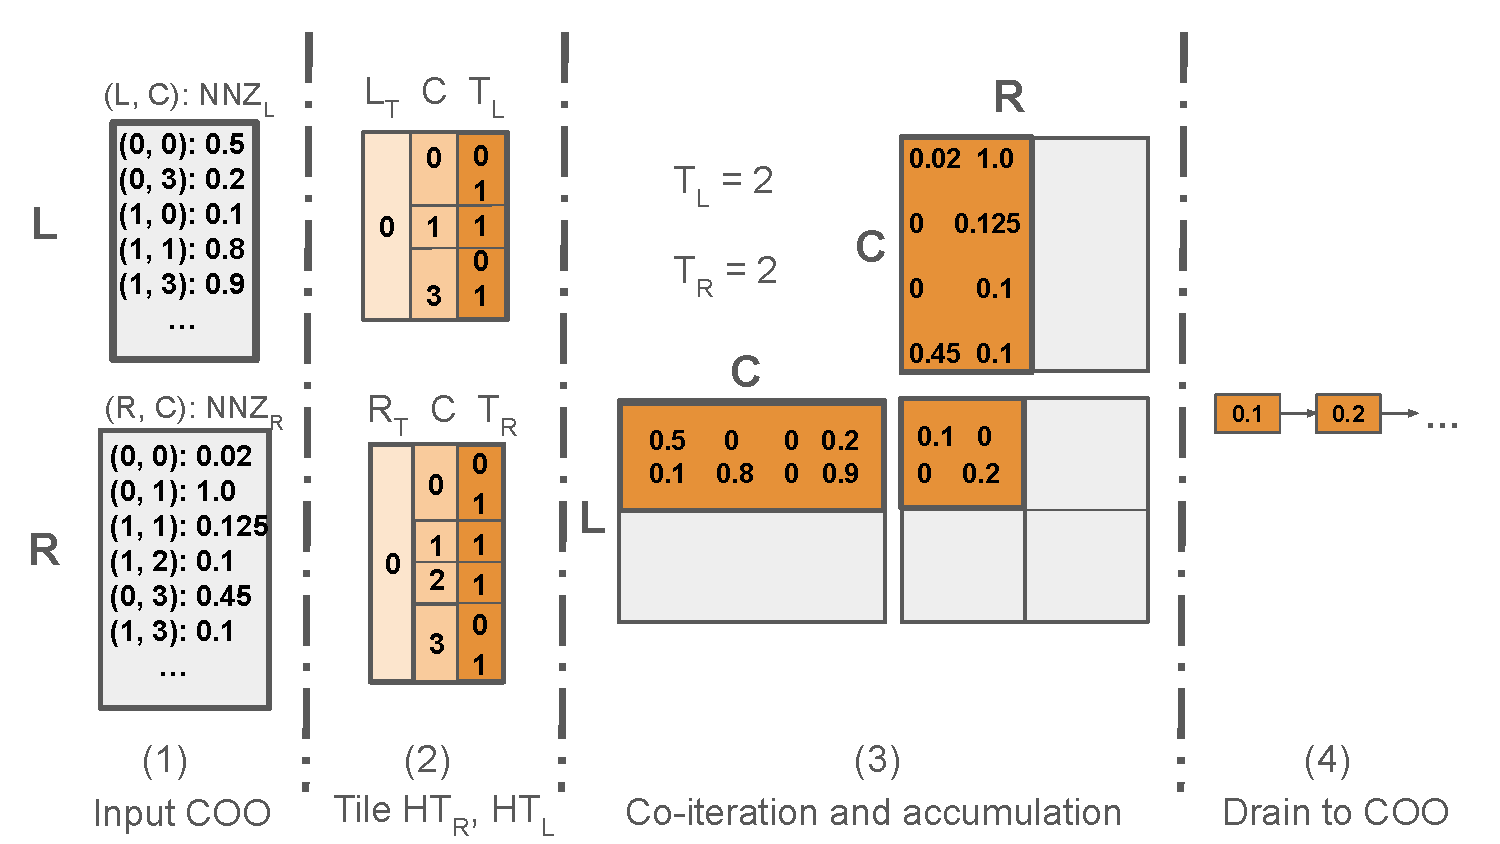
\includegraphics[scale=0.35]{fastcc system diag.pdf}
\caption{Intermediate steps of the FaSTCC contraction.}
\label{fig:frostt}
\end{figure}
% {\color{red} \bf We are no longer just Tiled CO; we have unified with CI; presentation of the algorithmic details need adaptation to match teh generalization.}
% The CO scheme described earlier (Algorithm~\ref{algo:co}) uses a 2D workspace $\mathit{WS}$ indexed by $l\in \mathbb{L}$ and $r\in \mathbb{R}$. Each workspace element 
% $\mathit{WS}(l,r)$ accumulates a series of contributions to output element $\mathit{Out}(l,r)$. 

In this section we present \ourtool, an efficient parallel implementation of a 2D-tiled CO scheme for sparse tensor contractions. As introduced in the previous section, the $\mathbb{L} \times \mathbb{R}$  index space of the output tensor is partitioned into ${\mathit{NL} \ast \mathit{NR}}$ tiles, where $\mathit{NL} = \lceil|\mathbb{L}| / \mathit{T_L} \rceil$ and $\mathit{NR} = \lceil|\mathbb{R}| / \mathit{T_R} \rceil$.

\subsection{Tiling and Workspace Design}
%\pp{We need a figure caption.}
%A key feature of our approach is that we define 2D tiling of index space $\mathbb{L} \times \mathbb{R}$ and use a workspace $\mathit{WS}$ that accumulates only the elements of that data tile of $\mathit{Out}$.
%This approach has two advantages. First, without tiling, the amount of memory needed for the workspace may become prohibitive. Second, tiling allows for improved data locality. 
%Both advantages are elaborated later in the paper and are illustrated with experimental studies [TODO: add discussion later]. 

%The tiling approach is parameterized by tile sizes $\mathit{TL}$ and $\mathit{TR}$.
%Later we discuss the considerations for choosing these tile sizes.
%For simplicity of presentation, we assume that $|\mathbb{L}|$ is a multiple of $\mathit{TL}$ (and similarly for $\mathit{TR}$). The handling of the general case with partial tiles is straightforward and not discussed due to space constraints. Let $\mathit{NL} = |\mathbb{L}| / \mathit{TL} $ and $\mathit{NR} = |\mathbb{R}| / \mathit{RL} $. 

\paragraph{Output tiles and input tiles}
Consider an output data tile $\mathit{Out}_{i,j}$ where $0\le i < \mathit{NL}$ and $0\le j < \mathit{NR}$. The tile is indexed by intra-tile indices $l$ and $r$ such that $0 \le l < \mathit{T_L}$ and $0 \le r < \mathit{T_R}$. Element $\mathit{Out}_{i,j}(l,r)$ corresponds to 
$\mathit{Out}(i\ast \mathit{T_L}+l,j \ast \mathit{T_R} + r)$. 

%[TODO: add a figure] 
To compute $\mathit{Out}_{i,j}$, we need a 1D tile $L_i$ of the left tensor $L$ and a 1D tile $R_j$ of the right tensor $R$. Here $L_i$ corresponds to elements $L(c,l)$ such that $i\ast \mathit{T_L} \le l < (i+1) \ast \mathit{T_L}$. Similarly, $R_j$ corresponds to elements $R(c,r)$ such that $j\ast \mathit{T_R} \le r < (j+1) \ast \mathit{T_R}$. To reflect this tiling of the inputs,
we represent the left input tensor using $\mathit{NL}$ hash tables of the form 
$$\mathit{HL}_i: \mathbb{C} \rightarrow \mathcal{P}(\{ 0, \ldots, \mathit{T_L} -1\} \times \mathbb{V})$$ 
and the right input tensor using $\mathit{NR}$ hash tables of the form 
$$\mathit{HR}_j: \mathbb{C} \rightarrow \mathcal{P}(\{ 0, \ldots, \mathit{T_R} -1\} \times \mathbb{V})$$ 
Map $\mathit{HL}_i$ represents input tile $L_i$ while $\mathit{HR}_j$ represents input tile $R_j$. The maps store intra-tile indices for the non-contraction data dimensions, together with the corresponding non-zero data values. For example, each $\langle l,\mathit{lv} \rangle \in \mathit{HL}_i(c)$ corresponds to an input element $L(c,i\ast \mathit{T_L}+l)$ with value $\mathit{lv}$. 

\paragraph{\ourtool \ algorithm} At the outermost level, Algorithm~\ref{algo:fastcc} iterates over output tiles $\mathit{Out}_{i,j}$. 
%Note that this iteration can be done in parallel, as discussed later [TODO: add discussion later]. 
For every $c$ such that both 
$\mathit{HL}_i$ and $\mathit{HR}_j$ contain some non-zero elements for $c$, the workspace $\mathit{WS}$ accumulates the contributions to $\mathit{Out}_{i,j}$ due to $c$. The output tile is then ``drained'' to the output tensor, with appropriate remapping of intra-tile indices $l$ and $r$. 
%This draining can also zero out the corresponding workspace elements, in preparation for the next iteration of the $j$ loop.

\begin{algorithm}[h]
\DontPrintSemicolon
\LinesNumbered
\For{$i \gets 0$ \KwTo $\mathit{NL} - 1$}{
\For{$j \gets 0$ \KwTo $\mathit{NR} - 1$}{
$\mathit{WS} \gets \emptyset$ \;
\For{$c \in \mathit{HL}_i.\mathit{keys}$}{
\If{$c \in \mathit{HR}_j.\mathit{keys}$}{
  \For{$\langle l,\mathit{lv} \rangle \in \mathit{HL}_i(c)$}{
    \For{$\langle r,\mathit{rv} \rangle \in \mathit{HR}_j(c)$}{ 
        $\mathit{WS}.\mathit{upsert}(l,r,\mathit{lv} \ast \mathit{rv})$ \;
}
}
}
}
\For{$\langle l, r \rangle \in \mathit{WS}.\mathit{keys}$}{
$\mathit{Out}.\mathit{append}(i\ast \mathit{T_L}+l,j \ast \mathit{T_R} + r, \mathit{WS}(l,r))$
}
% OLD VERSION
%\For{$c \in \mathbb{C}$}{
%  $\mathit{WS} \gets \emptyset$ \;
%  \For{$\langle l,\mathit{lv} \rangle \in \mathit{HL}_i(c)$}{
%    \For{$\langle r,\mathit{rv} \rangle \in \mathit{HR}_j(c)$}{ 
%        $\mathit{WS}.\mathit{upsert}(l,r,\mathit{lv} \ast \mathit{rv})$ \; } }
%          \For{$\langle l, r \rangle \in \mathit{WS}.\mathit{keys}$}{
%    $\mathit{Out}.\mathit{append}(l, r, \mathit{WS}(l,r))$ } }
    }}
\caption{\ourtool\ contraction\label{algo:fastcc}}
\end{algorithm}


\subsection{Implementation Details and Parallelization Techniques}
The \ourtool\ contraction has four steps: (1) construction of maps $\mathit{HL}_i$ and $\mathit{HR}_j$, (2) iteration over matching positions of $\mathit{HL}_i$ and $\mathit{HR}_j$,  (3) accumulation of partial results in the workspace, and (4) draining the workspace into the output COO list. Next we describe the parallel implementation of each of these steps individually.


\paragraph{Parallel construction of hash tables} Recall that non-zero elements of the left operand tensor $L$
are represented via hash tables $\mathit{HL}_i : \mathbb{C} \rightarrow \mathcal{P}(\{ 0, \ldots, \mathit{T_L} -1\} \times \mathbb{V})$. 
Each element $L(l, c)$ with value $\mathit{lv}$ is represented in map $\mathit{HL}_i$, where $i = \left \lfloor{l/\mathit{T_L}} \right \rfloor$, such that set $\mathit{HL}_i(c)$ contains a pair with the intra-tile index (e.g., $l\bmod \mathit{T_L}$) and the value $\mathit{lv}$. The representation of the right operand $R$ is similar.
This is illustrated in Figure~\ref{fig:frostt}, step 2 (tile hash tables). The example shows the computation of one output tile.
%In the example the number of tiles, $T_L = T_R = 2$. Only tile $L_T = R_T = 0$ is shown. $L$ from the original tensor maps directly to $T_L$.

Construction of these hash tables is performed in parallel.
Half the threads work on $\mathit{HL}$ while the other half works on $\mathit{HR}$.
This is implemented using OpenMP parallel regions with nested parallelism.
Each thread in the left team reads the input tensor $L$ in parallel, adding any points that are inside the thread's tile spaces to thread-local hash tables.
For example, thread $0$ in the left team is responsible for constructing all $\mathit{HL}_i$ with $i \bmod \mathit{num\_threads} = 0$, thread $1$ builds all $\mathit{HL}_i$ with $i \bmod \mathit{num\_threads} = 1$, and so on. 

\paragraph{Parallel co-iteration over $\mathit{HL}_i$ and $\mathit{HL}_j$}
We parallelize the co-iteration using a task queue.
Each tile-tile contraction (i.e., each combination of $i$ and $j$ values that computes some output tile $\mathit{Out}_{i,j}$ in Algorithm~\ref{algo:fastcc}) is defined as a separate task. These tasks are embarrassingly parallel, as each tile from the inputs is read-only, and each pair of input tiles \{$i$, $j$\} uniquely writes one tile of output.
Furthermore, since tasks are mapped to threads at run time, load imbalance is much lower than it would have been if we partitioned the index space of the non-zero elements. We use Taskflow for implementing this task queue \cite{taskflow}.


\paragraph{Parallel accumulation of partial results}
The result of this contraction is accumulated into a thread-local tile $\mathit{WS}_t$.
Based on an approach described later in Section~\ref{sec:model}, this can either be dense or sparse workspace.
At the end of the accumulation, $\mathit{WS}_t$ is drained into a thread-local COO linked list.

A dense tile structure includes:
(1) a buffer $\mathit{nnz}$ of size $\mathit{T_L} \ast \mathit{T_R} $ to hold non-zero elements of the tile, (2) a buffer 
$\mathit{apos}$ of the same size to hold integers corresponding to the active positions in the tile, and 
(3) a bitmask $\mathit{bm}$ with $\frac{\mathit{T_L} \ast \mathit{T_R}}{8}$ bits.
An update at position $p$ to this tile performs the following operations:
\begin{enumerate}
    \item Test and set bit $p$ of bitmask $\mathit{bm}$
    \item If the initial value of $\mathit{bm[p]}$ was $0$, append $\mathit{p}$ to $\mathit{apos}$
    \item Update the non-zero element at $\mathit{nnz[p]}$ with the new value
\end{enumerate}
The update operation takes constant time, and requires three random accesses to dense spaces.
In case the accumulator is sparse, we use an open addressed hash table and the update operation lowers to an upsert operation on the hash table, which is expected to execute in constant time.
This is shown in Figure~\ref{fig:frostt}, step 3, where the tile output data is computed from the input tile hash tables.

\paragraph{Parallel drain from tiles to COO output}
Once the tile has been filled with data,
the thread that owns that tile has to write the data to the COO list before working on the next tile.
In case the tile is a sparse accumulator, the thread simply iterates over the underlying hash table and appends to the COO list each non-zero with key as co-ordinate and value as the data.

For dense tiles, we use array $\mathit{apos}$ to perform the drain faster.
The thread iterates over this array of active non-zero positions within the tile.
It reads the non-zero elements from array $\mathit{nnz}$ with positions as given in $\mathit{apos}$, i.e. $\mathit{nnz[apos[iter]]}$, and appends them to the COO list.
Therefore, we iterate only over the non-zeros instead of iterating over the entire dense tile area of size $\mathit{T_L} \ast \mathit{T_R}$.
This is shown in Figure \ref{fig:frostt}, step 4 (drain to output COO) where the non-zeros from the tile are extracted and stored in the COO linked list.

\paragraph{COO representation for the output}
With the above four steps, we construct one COO list per thread that represents disjoint sets of the sparse tensor data.
The master thread concatenates these disjoint thread-local lists
using pointer movements (no data copies) into one output COO result.
We implement a memory pool layer to make the COO construction faster.
Each thread gets heap allocations in chunks of 512MB as it pushes non-zeros to the thread-local COO.
As the threads complete, they free up their local heap allocations.


%Recall from Algorithm~\ref{algo:tiled-co} that a workspace $\mathit{WS}$ is used to accumulate contributions to an output data tile $\mathit{Out}_{i,j}$ for each pair of values of outer iterators $i$ and $j$. We consider two approaches for 
%the design of this workspace. 

%When using a \emph{dense workspace}, a contiguous buffer with $\mathit{TL} \ast \mathit{TR}$ floating-point values can be used. For any $l$ and $r$, $\mathit{WS}.\mathit{upsert}(l,r,\mathit{lv} \ast \mathit{rv})$ updates the corresponding value in the buffer. In this case, the workspace should be zeroed out at the start of each iteration of the $j$ loop from Algorithm~\ref{algo:tiled-co}.
%This ``reset'' is performed at the end of the previous $j$ iteration: whenever a workspace element is appended to $\mathit{Out}$, it is immediately reset to a zero value. 
%[TODO: how do we know which elements of the dense workspace have been touched?]

%An alternative approach that reduces memory consumption is to implement $\mathit{WS}$ with a hash map; we refer to this 
%choice as a \emph{sparse workspace}. When the output data tiles are very sparse, a sparse workspace 
%can achieve significant memory savings. As a consequence, this makes it possible to increase the tile size significantly without running out of memory. In the next section, we discuss a performance modeling approach that further characterizes the trade-offs of these two choices, together with the considerations for selecting corresponding tile sizes. 


%\input{details-old}
%\input{model}
\section{Figures from the paper evaluation}


\begin{figure*}%[t]
    \ref{barLegend}\\
    \centering
    %\begin{subfigure}{\columnwidth}

\begin{tikzpicture}
  \centering
  \begin{axis}[
    barChartSmall,
    legend to name=barLegend,
    symbolic x coords={Chicago-0, Chicago-01, Chicago-123, Vast-5d-01, Vast-5d-014, Uber-02, Uber-123, NIPS-2, NIPS-23,NIPS-013},
    enlarge x limits=0.15,
    ]

    %BETA OuroborosPVA OuroborosCS
    \addplot[draw=none, OrangeBarStyle, x=tensor, y=speedup]   table {data/speedup_best_desktop.txt};
    %\addplot[draw=none, fill=green!30, x=op, y=perf]   table {data/orkut_CUDA.txt};
    
    \addplot[draw=none, BlueBarStyle, x=tensor, y=speedup]   table {data/speedup_model_desktop.txt};
   
    \legend{Speedup: best tile size, Speedup: model-based size};
  \end{axis}
  \end{tikzpicture}
  %Found it! was the semicolon;
  \caption{FROSTT comparison on Desktop machine with 8 threads}
  \label{fig:DesktopBarFigure}
\end{subfigure}%
    \begin{subfigure}{\columnwidth}

\begin{tikzpicture}
  \centering
  \begin{axis}[
    barChartSmall,
    legend to name=barLegend,
    symbolic x coords={Chicago-0, Chicago-01, Chicago-123, Vast-5d-01, Vast-5d-014, Uber-02, Uber-123, NIPS-2, NIPS-23,NIPS-013},
    enlarge x limits=0.15,
    ]

    \addplot[draw=none, OrangeBarStyle, x=tensor, y=speedup]   table[col sep=comma] {data/speedup_best_server.txt};
    %\addplot[draw=none, fill=green!30, x=op, y=perf]   table {data/orkut_CUDA.txt};
    
    \addplot[draw=none, BlueBarStyle, x=tensor, y=speedup]   table[col sep=comma] {data/speedup_model_server.txt};

    
    \legend{Speedup: best tile size, Speedup: model-based size};
  \end{axis}
  \end{tikzpicture}
  %Found it! was the semicolon;
  \caption{FROSTT comparison on your machine.}
  \label{fig:ServerpBarFigure}
\end{subfigure}
    
    %\begin{subfigure}{\columnwidth}

\begin{tikzpicture}
  \centering
  \begin{axis}[
    barChartSmall,
    legend to name=moleculeDesktopLegend,
    symbolic x coords={Caffeine-ovov, Caffeine-vvoo, Caffeine-vvov, Guanine-ovov, Guanine-vvoo, Guanine-vvov},
    enlarge x limits=0.15,
    ]


    %BETA OuroborosPVA OuroborosCS
    \addplot[draw=none, OrangeBarStyle, x=tensor, y=speedup]   table {data/molecules/desktop_best.txt};
    %\addplot[draw=none, fill=green!30, x=op, y=perf]   table {data/orkut_CUDA.txt};

    \addplot[draw=none, BlueBarStyle, x=tensor, y=speedup]   table {data/molecules/desktop_model.txt};

    \legend{Speedup: best tile size, Speedup: model-based size};
  \end{axis}
  \end{tikzpicture}
  %Found it! was the semicolon;
  \caption{Quantum chemistry comparison on desktop machine with 8 threads.}
  \label{fig:moleculesDesktop}
\end{subfigure}%
    \begin{subfigure}{\columnwidth}

\begin{tikzpicture}
  \centering
  \begin{axis}[
    barChartSmall,
    symbolic x coords={caffeine-ovov, caffeine-vvoo, caffeine-vvov, guanine-ovov, guanine-vvoo, guanine-vvov},
    enlarge x limits=0.15,
    ]


    %BETA OuroborosPVA OuroborosCS
    \addplot[draw=none, OrangeBarStyle, x=tensor, y=speedup]   table[col sep=comma] {data/molecules/server_best.txt};
    %\addplot[draw=none, fill=green!30, x=op, y=perf]   table {data/orkut_CUDA.txt};

    \addplot[draw=none, BlueBarStyle, x=tensor, y=speedup]   table[col sep=comma] {data/molecules/server_model.txt};

  \end{axis}
  \end{tikzpicture}
  %Found it! was the semicolon;
  \caption{Quantum chemistry comparison on your machine.}
  \label{fig:moleculesServer}
\end{subfigure}
    \caption{Speedups over Sparta, with the best and model-chosen tile sizes on the FROSTT and quantum chemistry benchmarks.}
    \label{fig::all_comparisons}
    \end{figure*}


% \begin{figure}%[t]
    \ref{barLegend}
    \centering
    %\begin{subfigure}{\columnwidth}

\begin{tikzpicture}
  \centering
  \begin{axis}[
    barChartSmall,
    legend to name=barLegend,
    symbolic x coords={Chicago-0, Chicago-01, Chicago-123, Vast-5d-01, Vast-5d-014, Uber-02, Uber-123, NIPS-2, NIPS-23,NIPS-013},
    enlarge x limits=0.15,
    ]

    %BETA OuroborosPVA OuroborosCS
    \addplot[draw=none, OrangeBarStyle, x=tensor, y=speedup]   table {data/speedup_best_desktop.txt};
    %\addplot[draw=none, fill=green!30, x=op, y=perf]   table {data/orkut_CUDA.txt};
    
    \addplot[draw=none, BlueBarStyle, x=tensor, y=speedup]   table {data/speedup_model_desktop.txt};
   
    \legend{Speedup: best tile size, Speedup: model-based size};
  \end{axis}
  \end{tikzpicture}
  %Found it! was the semicolon;
  \caption{FROSTT comparison on Desktop machine with 8 threads}
  \label{fig:DesktopBarFigure}
\end{subfigure}
    \begin{subfigure}{\columnwidth}

\begin{tikzpicture}
  \centering
  \begin{axis}[
    barChartSmall,
    legend to name=barLegend,
    symbolic x coords={Chicago-0, Chicago-01, Chicago-123, Vast-5d-01, Vast-5d-014, Uber-02, Uber-123, NIPS-2, NIPS-23,NIPS-013},
    enlarge x limits=0.15,
    ]

    \addplot[draw=none, OrangeBarStyle, x=tensor, y=speedup]   table[col sep=comma] {data/speedup_best_server.txt};
    %\addplot[draw=none, fill=green!30, x=op, y=perf]   table {data/orkut_CUDA.txt};
    
    \addplot[draw=none, BlueBarStyle, x=tensor, y=speedup]   table[col sep=comma] {data/speedup_model_server.txt};

    
    \legend{Speedup: best tile size, Speedup: model-based size};
  \end{axis}
  \end{tikzpicture}
  %Found it! was the semicolon;
  \caption{FROSTT comparison on your machine.}
  \label{fig:ServerpBarFigure}
\end{subfigure}
    
    % \ref{frosttScalingLegend}
    % \begin{subfigure}{\columnwidth}

\begin{tikzpicture}
  \centering
  \begin{axis}[
    barChart,
    legend to name=frosttScalingLegend,
    symbolic x coords={1,2,4,8,16,32,64},
    enlarge x limits=0.15,
    ]

    %BETA OuroborosPVA OuroborosCS
    \addplot[draw=none, OrangeBarStyle, x=threads, y=speedup]   table {data/chicago0_threadscale.txt};
    %\addplot[draw=none, fill=green!30, x=op, y=perf]   table {data/orkut_CUDA.txt};
    
    \addplot[draw=none, BlueBarStyle, x=threads, y=speedup]   table {data/caffeinevvov_threadscale.txt};
   
  
  \legend{Chicago mode 0, caffeine vvov};
  \end{axis}
  \end{tikzpicture}
  %Found it! was the semicolon;
  \caption{Factor improvement over single thread execution for the FaSTCC kernel from 1 to 64 threads.}
  \label{fig:chic0_threadscale}
\end{subfigure}
    \caption{Speedups over Sparta, with the best and model-chosen tile sizes, for the FROSTT benchmarks.}
    \label{fig::barFigures}
\end{figure}

% \begin{figure}[t]
    \ref{moleculeDesktopLegend}
    \centering
    \begin{subfigure}{\columnwidth}

\begin{tikzpicture}
  \centering
  \begin{axis}[
    barChartSmall,
    legend to name=moleculeDesktopLegend,
    symbolic x coords={Caffeine-ovov, Caffeine-vvoo, Caffeine-vvov, Guanine-ovov, Guanine-vvoo, Guanine-vvov},
    enlarge x limits=0.15,
    ]


    %BETA OuroborosPVA OuroborosCS
    \addplot[draw=none, OrangeBarStyle, x=tensor, y=speedup]   table {data/molecules/desktop_best.txt};
    %\addplot[draw=none, fill=green!30, x=op, y=perf]   table {data/orkut_CUDA.txt};

    \addplot[draw=none, BlueBarStyle, x=tensor, y=speedup]   table {data/molecules/desktop_model.txt};

    \legend{Speedup: best tile size, Speedup: model-based size};
  \end{axis}
  \end{tikzpicture}
  %Found it! was the semicolon;
  \caption{Quantum chemistry comparison on desktop machine with 8 threads.}
  \label{fig:moleculesDesktop}
\end{subfigure}
    \begin{subfigure}{\columnwidth}

\begin{tikzpicture}
  \centering
  \begin{axis}[
    barChartSmall,
    symbolic x coords={caffeine-ovov, caffeine-vvoo, caffeine-vvov, guanine-ovov, guanine-vvoo, guanine-vvov},
    enlarge x limits=0.15,
    ]


    %BETA OuroborosPVA OuroborosCS
    \addplot[draw=none, OrangeBarStyle, x=tensor, y=speedup]   table[col sep=comma] {data/molecules/server_best.txt};
    %\addplot[draw=none, fill=green!30, x=op, y=perf]   table {data/orkut_CUDA.txt};

    \addplot[draw=none, BlueBarStyle, x=tensor, y=speedup]   table[col sep=comma] {data/molecules/server_model.txt};

  \end{axis}
  \end{tikzpicture}
  %Found it! was the semicolon;
  \caption{Quantum chemistry comparison on your machine.}
  \label{fig:moleculesServer}
\end{subfigure}
    \caption{Speedups over Sparta, with the best and model-chosen tile sizes for the quantum chemistry benchmarks.}
    \label{fig::molecules}
    \end{figure}


% \begin{figure}[t]
    %\ref{barLegend}
    \centering
    
    \ref{frosttScalingLegend}
    %\begin{subfigure}{\columnwidth}

\begin{tikzpicture}
  \centering
  \begin{axis}[
    barChart,
    legend to name=frosttScalingLegend,
    symbolic x coords={1,2,4,8,16,32,64},
    enlarge x limits=0.15,
    ]

    %BETA OuroborosPVA OuroborosCS
    \addplot[draw=none, OrangeBarStyle, x=threads, y=speedup]   table {data/chicago0_threadscale.txt};
    %\addplot[draw=none, fill=green!30, x=op, y=perf]   table {data/orkut_CUDA.txt};
    
    \addplot[draw=none, BlueBarStyle, x=threads, y=speedup]   table {data/caffeinevvov_threadscale.txt};
   
  
  \legend{Chicago mode 0, caffeine vvov};
  \end{axis}
  \end{tikzpicture}
  %Found it! was the semicolon;
  \caption{Factor improvement over single thread execution for the FaSTCC kernel from 1 to 64 threads.}
  \label{fig:chic0_threadscale}
\end{subfigure}
    \begin{tikzpicture}
  \centering
  \begin{axis}[
    barChartScaling,
    legend to name=frosttScalingLegend,
    symbolic x coords={1,2,4,8,16,32,64},
    enlarge x limits=0.15,
    ]

    %BETA OuroborosPVA OuroborosCS
    \addplot[draw=none, OrangeBarStyle, x=threads, y=speedup]   table {data/chicago0_threadscale.txt};
    %\addplot[draw=none, fill=green!30, x=op, y=perf]   table {data/orkut_CUDA.txt};
    
    \addplot[draw=none, BlueBarStyle, x=threads, y=speedup]   table {data/caffeinevvov_threadscale.txt};
   
  
  \legend{Chicago mode 0, Caffeine vvov};
  \end{axis}
  \end{tikzpicture}
  %Found it! was the semicolon;
  \caption{Factor improvement in run-time over single thread execution for the FaSTCC kernel from 1 to 64 threads.}
  \label{fig:chic0_threadscale}
\end{figure}


% \begin{table}[htb]
% \caption{Model output for each experiment. First column is tensor name and contraction mode (in subscript). Time for dense contraction is shown as $\mathit{Time}_D$, similarly for sparse. Model prediction for dense vs sparse accumulator is shown in column (D/S).}
% {\small
% \begin{tabular}{|l|r|r|r|l|l|l|}
% \hline
% \multicolumn{1}{|c|}{\multirow{2}{*}{\textbf{Tensor}}} & \multicolumn{1}{c|}{\multirow{2}{*}{\textbf{$\mathit{p_L}$(\%)}}} & \multicolumn{1}{c|}{\multirow{2}{*}{\textbf{$\mathit{p_R}$(\%)}}} & \multicolumn{1}{l|}{\multirow{2}{*}{\textbf{$\mathit{E_{\mathit{nnz}}(T^2)}$}}} & \multirow{2}{*}{\textbf{$\mathit{Time}_D$}} & \multirow{2}{*}{\textbf{$\mathit{Time}_S$}} & \multirow{2}{*}{\textbf{D/S}} \\
% \multicolumn{1}{|c|}{} & \multicolumn{1}{c|}{} & \multicolumn{1}{c|}{} & \multicolumn{1}{l|}{} &  &  &  \\ \hline
% \textbf{chic$_0$} & 1.46 & 1.46 & 4.79E+04 & 9.21 & 9.36 & D \\ \hline
% \textbf{chic$_{01}$} & 1.46 & 1.46 & 65536 & 0.33 & 0.54 & D \\ \hline
% \textbf{chic$_{123}$} & 1.46 & 1.46 & 6.55E+04 & 1.23 & 2.06 & D \\ \hline
% \textbf{uber$_{02}$} & 0.04 & 0.04 & 2.00E+03 & 0.55 & 0.73 & D \\ \hline
% \textbf{uber$_{123}$} & 0.04 & 0.04 & 6.55E+04 & 0.34 & 0.38 & D \\ \hline
% \textbf{vast$_{01}$} & 7.78E-06 & 7.78E-06 & 7.38E+00 & 4.23 & 4.26 & D \\ \hline
% \textbf{vast$_{014}$} & 7.78E-06 & 7.78E-06 & 6.54E+02 & 4.36 & 4.45 & D \\ \hline
% \textbf{NIPS$_2$} & 1.83E-04 & 1.83E-04 & 3.08E-03 & DNF & 2.44 & S \\ \hline
% \textbf{NIPS$_{23}$} & 1.83E-04 & 1.83E-04 & 5.24E-02 & 0.73 & 0.259 & S \\ \hline
% \textbf{NIPS$_{013}$} & 1.83E-04 & 1.83E-04 & 2.65E+01 & 1.44 & 1.48 & D \\ \hline
% \textbf{G-ovov} & 0.63 & 0.63 & 1.98E+04 & 0.315 & 0.566 & D \\ \hline
% \textbf{G-vvoo} & 18.36 & 0.17 & 6.16E+04 & 11.28 & 12.12 & D \\ \hline
% \textbf{G-vvov} & 18.36 & 0.63 & 6.55E+04 & 36.09 & 85.91 & D \\ \hline
% \textbf{C-ovov} & 3.66 & 3.66 & 6.50E+04 & 0.219 & 0.566 & D \\ \hline
% \textbf{C-vvoo} & 41.90 & 1.03 & 6.55E+04 & 3.79 & 4.305 & D \\ \hline
% \textbf{C-vvov} & 41.90 & 3.66 & 65536 & 16.03 & 107.4 & D \\ \hline
% \end{tabular}
% }
% \label{tab:prob_frostt}
% \end{table}

\begin{figure}[h]
    \ref{frosttScatterLegend}
    \centering
    \begin{subfigure}{\columnwidth}
\pgfplotstableread[col sep=comma,]{data/main_scatter.txt}\datatable
\begin{tikzpicture}
\begin{axis}[
    ScatterPlot,
    %xticklabels from table={\datatable}{Bytes},
    xmode=log,
    ymode=log,
    legend to name=frosttScatterLegend,
    legend columns = 4,
    legend style={font=\small},
    ]


    %NIPS-013	Chicago-0	Chicago-01	Chicago-123	Vast-5d-01	Vast-5d-014	Uber-02	Uber-123

    \addplot[NIPS013] table [x=tile, y=NIPS-013]{\datatable};
    \addlegendentry{NIPS-013}

    \addplot[Chicago0] table [x=tile, y=Chicago-0]{\datatable};
    \addlegendentry{Chicago-0}

    \addplot[Chicago01] table [x=tile, y=Chicago-01]{\datatable};
    \addlegendentry{Chicago-01}

    \addplot[Chicago123] table [x=tile, y=Chicago-123]{\datatable};
    \addlegendentry{Chicago-123}

    \addplot[Vast01] table [x=tile, y=Vast-5d-01]{\datatable};
    \addlegendentry{Vast-5d-01}

    \addplot[Vast014] table [x=tile, y=Vast-5d-014]{\datatable};
    \addlegendentry{Vast-5d-014}

    \addplot[Uber02] table [x=tile, y=Uber-02]{\datatable};
    \addlegendentry{Uber-02}

    \addplot[Uber123] table [x=tile, y=Uber-123]{\datatable};
    \addlegendentry{Uber-123}
    
    % \addplot[Cuda] table [x=Bytes, y=CUDA]{\datatable};
    % \addlegendentry{CUDA}








\end{axis}
\end{tikzpicture}


\caption{Execution time variation with tile size: FROSTT}
\label{fig:frostt_scatter_subfig}

\end{subfigure}

    \ref{moleculeScatterLegend}
    \begin{subfigure}{\columnwidth}
\pgfplotstableread[col sep=comma,]{data/molecule_scatter.txt}\datatable
\begin{tikzpicture}
\begin{axis}[
    moleculeScatterPlot,
    %xticklabels from table={\datatable}{Bytes},
    xmode=log,
    ymode=log,
    legend to name=moleculeScatterLegend,
    legend columns = 3,
    legend style={font=\small},
    ]



    %Caffeine-vvoo
    \addplot[NIPS013] table [x=tile, y=caffeine-vvoo]{\datatable};
    \addlegendentry{c-vvoo}

    %Caffeine-vvov
    \addplot[Chicago0] table [x=tile, y=caffeine-vvov]{\datatable};
    \addlegendentry{Caffeine-vvov}

    %Caffeine-ovov
    \addplot[Chicago01] table [x=tile, y=caffeine-ovov]{\datatable};
    \addlegendentry{Caffeine-ovov}

    %Guanine-vvoo
    \addplot[Chicago123] table [x=tile, y=guanine-vvoo]{\datatable};
    \addlegendentry{Guanine-vvoo}

    %Guanine-vvov
    \addplot[Vast01] table [x=tile, y=guanine-vvov]{\datatable};
    \addlegendentry{Guanine-vvov}

    %Guanine-ovov
    \addplot[Vast014] table [x=tile, y=guanine-ovov]{\datatable};
    \addlegendentry{Guanine-ovov}



\end{axis}
\end{tikzpicture}


\caption{Execution time variation with tile size: quantum chemistry}
\label{fig:frostt_u}
\label{fig:dlpno_u}
\label{fig:molecule_scatter_subfig}

\end{subfigure}
    %\caption{Scatter plots}
        \caption{Execution time as a function of tile size.}
    \label{fig::scatter}
\end{figure}


%\begin{figure}[t]
    \ref{tacoLegend}
    \centering
    \begin{subfigure}{\columnwidth}

\begin{tikzpicture}
  \centering
  \begin{axis}[
    tacoBarChart,
    legend to name=tacoLegend,
    symbolic x coords={Chicago-0, Chicago-01, Chicago-123, Vast-5d-01, Vast-5d-014, Uber-02, Uber-123, NIPS-2, NIPS-23,NIPS-013},
    enlarge x limits=0.15,
    ]

    %BETA OuroborosPVA OuroborosCS
    \addplot[draw=none, BlueBarStyle, x=tensor, y=slowdown]   table {data/taco_frostt.txt};
    \addplot[draw=none, OrangeBarStyle, x=tensor, y=slowdown]   table {data/sparta_frostt.txt};
    %\addplot[draw=none, fill=green!30, x=op, y=perf]   table {data/orkut_CUDA.txt};
    
   \legend{Improvement over TACO, Improvement over SPARTA};
  \end{axis}
  \end{tikzpicture}
  %Found it! was the semicolon;
  \caption{FROSTT benchmarks.}
  \label{fig::tacoFrostt}
\end{subfigure}

    \begin{subfigure}{\columnwidth}

\begin{tikzpicture}
  \centering
  \begin{axis}[
    tacoBarChart,
    symbolic x coords={Caffeine-ovov, Caffeine-vvoo, Caffeine-vvov, Guanine-ovov, Guanine-vvoo, Guanine-vvov},
    xticklabels={Caffeine-ovov, Caffeine-vvoo, Caffeine-vvov, Guanine-ovov, Guanine-vvoo, Guanine-vvov},
    enlarge x limits=0.15,
    ]

    %BETA OuroborosPVA OuroborosCS
    \addplot[draw=none, BlueBarStyle, x=tensor, y=slowdown]   table {data/taco_molecule.txt};
    \addplot[draw=none, OrangeBarStyle, x=tensor, y=slowdown]   table {data/sparta_molecule.txt};
    %\addplot[draw=none, fill=green!30, x=op, y=perf]   table {data/orkut_CUDA.txt};
    
   

  \end{axis}
  \end{tikzpicture}
  %Found it! was the semicolon;
  \caption{Quantum chemistry benchmarks.}
  \label{fig::tacoMolecule}
\end{subfigure}



    \caption{Speedups of \ourtool\ for sequential execution.}
    \label{fig:frostt_sequential}
    
\end{figure}



%\clearpage
\end{document}
\endinput
